Das Diagramm zeigt die Geschwindigkeit eines Körpers auf einer geraden Linie. Zur Zeit $t = 0$ ist er bei $s = 0$.
\begin{center}
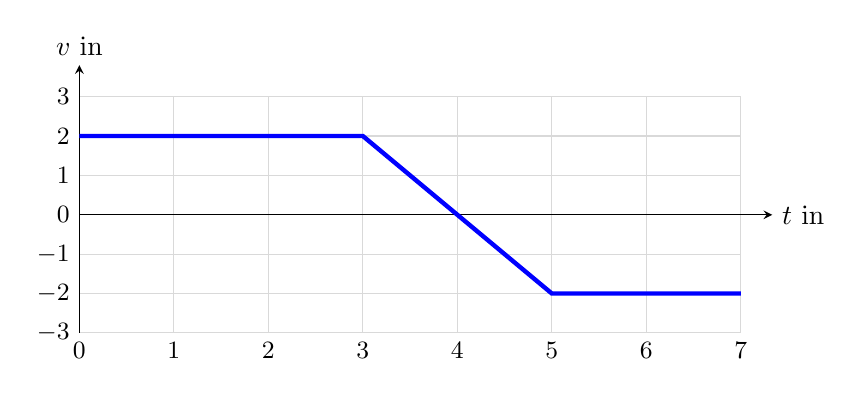
\begin{tikzpicture}[>=stealth, x=1.2cm, y=0.5cm]
 \draw[gray!30] (0,-3) grid[xstep=1, ystep=1] (7,3);
 \draw[->] (0,0) -- (7.333,0) node[right] {$t$ in \si{\second}};
 \draw[->] (0,-3) -- (0,3.8) node[above] {$v$ in \si{\meter\per\second}};
 \foreach \tk in {0,1,2,3,4,5,6,7} \node[below] at (\tk,-3) {\small $\tk$};
 \foreach \yk in {-3,-2,-1,0,1,2,3} \node[left] at (0,\yk) {\small $\yk$};
 \draw[ultra thick, blue] (0,2) -- (3,2) -- (5,-2) -- (7,-2);
\end{tikzpicture}
\end{center}
\begin{abcliste}
\abc Wann ist der Körper am weitesten vorne, und wo?
\abc \DuSie{Skizziere}{Skizzieren Sie} das $s(t)$-Diagramm von \SI{0}{\second} bis \tEO. Wo ist der Körper bei \tEO?
\end{abcliste}
